\documentclass[10pt]{article}
\usepackage{graphicx}
\usepackage{amsmath}
\usepackage{float}
\usepackage{subcaption}
\usepackage[margin=1in]{geometry}


\begin{document}
\pagenumbering{gobble}
\begingroup  
  \centering
  \large Fast \& Sparse Learning with Compositional Concept Training\\[1em]
  \small{Andrew Lampinen* (lampinen@stanford.edu, Department of Psychology, Stanford University),\\ James McClelland (mclelland@stanford.edu, Department of Psychollogy, Stanford University)}\par
\endgroup
\vspace{10pt}
The end-to-end training on large data sets that is customary for neural networks is very unlike the way that adult humans learn tasks. Humans can learn rapidly from few examples. In part, this is likely because humans can be taught to break problems down into smaller parts, and can utilize previously learned concepts. Previous work has shown that to learn very difficult tasks in neural networks, it is sometimes necessary to teach intermediate steps of the task (G{\"{u}l\c{c}ehre \& Bengio, 2013). Here, we suggest that even if a task is easily learnable in general, the technique of teaching intermediate steps to the network can lead to much better performance on sparse data sets, and faster learning on larger data sets.\par
We demonstrate this by teaching networks the rules to Conway's Game of Life: For a square surrounded by eight neighboring squares, a square with four or more live neighbors dies from overcrowding, and one with fewer than two live neighbors dies of loneliness. A living square with two or three live neighbors lives, and a dead square with three live neighbors becomes alive. This can be seen as a task of mapping from a 3 x 3 binary array (the current state) to a single binary value (life of the central unit at the next step). Alternatively, the task can be decomposed: First, evaluate the current life of a unit and the number of its living neighbors, and second, compute its life at the subsequent time-step from these features. We trained what we call a ``compositional'' network by training a single-layer (ReLU) network with 2 output units, one for number of neighbors (integer-valued target in the range $[0,8]$) and one for life of the central square (target -1 or 1), and simultaneously training a single hidden-layer (tanh) network to compute the life value at the next step from these unit's outputs. We compared this compositional network to a variety of standard neural networks (one with two hidden layers, first ReLU, second tanh, to parallel the compositional, and two networks with one of these hidden layers removed). The standard networks were trained to map the input array directly to the life value output. (See Figure \ref{networkdiagram} for a comparison of our network to the two hidden layer standard network.) All training was done by stochastic gradient descent using mean-squared error (learning rate=0.01, learning rate decay=0.99/epoch). To explore the networks' performance, we varied the number of training examples. Since there are 512 possible input arrays, we trained on $n$ of them (randomly selected on each run), and tested on the held out $512-n$. We conducted 100 runs each for $n = 64$ and $n=256$.\par
We found that the compositional network is able to learn from much sparser datasets than the standard networks. See Fig. \ref{n64figure} for a plot of test error rate, averaged across 100 runs, with $n = 64$ training examples chosen randomly on each run. Note that the average error rates do not quite reach zero; even the compositional network was not always successful at learning the task with $n = 64$. Furthermore, even with training sets sufficient for the standard networks to learn ($n = 256$, Fig. \ref{n256figure}), the compositional network learned the task much more rapidly. We conclude that learning explicit compositions of subtasks can offer benefits for sparse learning, and for rapid learning even on large data sets, likely by constraining the solution space which must be searched. These training approaches may lead to more human-like learning from neural networks.
\begin{figure}[H]
    \centering
    \begin{subfigure}[c]{0.35\textwidth}
	\centering
	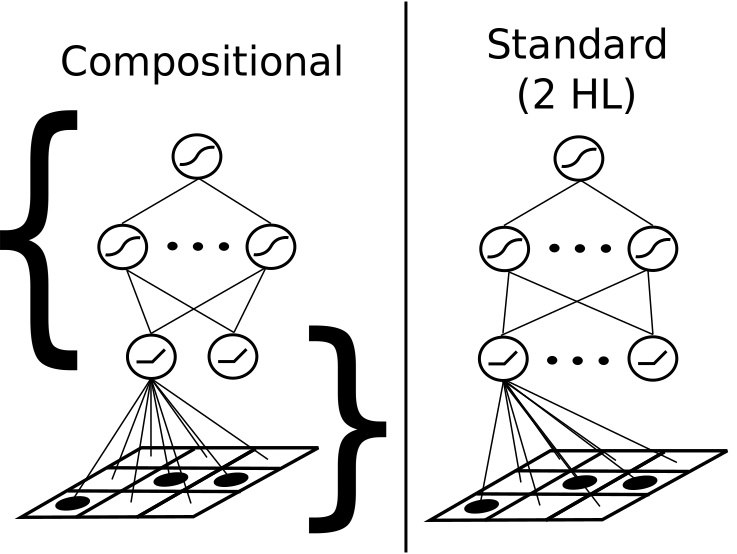
\includegraphics[width=0.9\textwidth]{figures/hierarchical_NN_abstract_figure.png}
	\caption{Network comparison (brackets in compositional network denote the sub-networks we trained. All hidden layers had 10 units.)}
	\label{networkdiagram}
    \end{subfigure}
    \begin{subfigure}[c]{0.3\textwidth}
	\centering
	\includegraphics[width=\textwidth]{figures/n64figure.png}
	\caption{Error rates for $n = 64$}
	\label{n64figure}
    \end{subfigure}
    \begin{subfigure}[c]{0.3\textwidth}
	\centering
	\includegraphics[width=\textwidth]{figures/n256figure.png}
	\caption{Error rates for $n = 256$}
	\label{n256figure}
    \end{subfigure}
    \caption{Network comparison \& results}
\end{figure}

\end{document}
